\newpage
\subsection{Clasificación de imágenes naturales}

	Para poder comprender de mejor manera la sección \ref{subsection: wang_recon_caracteres}, es necesario adentrarse en las particularidades que caracterízan a las imágenes naturales. Dado que, como se ha detallado anteriormente, no es sencillo trabajar con este tipo de imágenes, la siguiente sub-sección se enfoca en las características de las escenas naturales. Las siguientes sub-secciones van a explicar conceptos como el de gradiente que es necesario para poder entender a los descriptores HOG (ver \ref{subsection:hog}) usados tanto por Wang et. al. en \cite{wang}, como por el presente trabajo. Finalmente, se explica el proceso de binarización, necesario para poder usar el clasificador \textit{Random Ferns}.

	\subsubsection{Características}

Las características en las imágenes naturales son muy variadas. Dentro de las mismas podemos encontrar las variaciones de intensidad en la iluminación, la resolución, el ángulo en el que son tomadas, el fondo, las texturas, entre otros. Mas específicamente, dependiendo del objeto que se esté analizando, por ejemplo, texto, surgen más características como el tipo de fuente, el tamaño, la posición y orientación de los caracteres, la contaminación que pueda llegar a tener el texto por suciedad u oclusión, etc. La infita variedad que es posible encontrar en este tipo de imágenes, dificultan el trabajo de reconocimiento sobre ellas por lo que, en general, es necesario realizar un pre-procesamiento antes de usarlas.

	En el caso del reconocimiento de texto, dada la gran cantidad de formas en que se puede encontrar la imagen de un carácter, es necesario encontrar algún método que extraiga las características mas representativas para poder distinguilo. Para poder analizar los caracteres en las imágenes naturales, uno de los enfoques que adoptan Wang et al. en \cite{wang} es el de trabajar con el descriptor HOG de cada imagen. Para poder entender que es un descriptor HOG (que se detalla en \ref{subsection:hog}), primero es necesario comprender el concepto de gradiente que se explica a continuación.
	
	%	Desde la aparición de las primeras fotografías, las personas han buscado ``inmortalizar'' escenas, objetos o personas, con el objetivo de, en el area de la ciencias, extraer información útil de las mismas que pueda ser utilizada para su analisis o estudio. Con el surgimiento de los primeros formatos digitales, la necesidad pasó por encontrar métodos automáticos que permitieran clasificar y reconocer elementos dentro de las imágenes. Desde reconocer texto manuscrito, texto en carteles publicitarios, patentes, personas, animales hasta identificar zonas con agua en una imagen satelital. La cantidad de potenciales aplicaciones que se pueden obtener es enorme. Es por eso que en campos de investigación como visión por computadora, este es un tema de interés. Sin embargo, la clasificación en imágenes naturales no es una tarea para nada sencilla. Por ejemplo, en el reconocimiento de texto, las imágenes naturales contienen muchas información ``extra'' que se tiene que tener en cuenta. Ya sea la existencia de otros objetos ajenos a la clasificación, es decir, elementos que no son texto como así también variaciones propias en las características de la misma imagen (se detallan más adelante en esta sección).
	
	Hoy en día se ha avanzado mucho en el área de la clasificación en escenas naturales. Se han desarrollado muchas aplicaciones como aquellas capaces de reconocer personas \cite{DT05}, hasta las que pueden identificar patentes \cite{DAB}. Si bien dichos avances muestran que es posible realizar lo mismo en diferentes ámbitos, en otros como el reconocimiento de texto sigue siendo un desafío (en contextos naturales).
	
	
\paragraph{Características} ~\\
	
	Las características en las imágenes naturales son muy variadas. Todas estas variaciones dificultan el trabajo sobre ellas por lo cual en general es necesario realizar un trabajo de pre-procesamiento antes de trabajar con las mismas. Las características que podemos encontrar en este tipo de imágenes son las variaciones de intensidad en la iluminación, la resolución, el ángulo en el que son tomadas las mismas, el fondo, las texturas, entre otros. Mas específicamente, dependiendo del objeto que se esté analizando, por ejemplo, texto, surgen más características como el tipo de fuente, el tamaño, la posición y orientación de los caracteres, la contaminación que pueda llegar a tener el texto por suciedad u oclusión, etc.
	
	Para poder analizar los caracteres en las imágenes naturales, uno de los enfoques que adoptan Wang et al. en \cite{wang} es el de trabajar con el descriptor HOG de cada imagen. Para poder entender que es un descriptor HOG (que se detalla más adelante), primero es necesario comprender el concepto de gradiente que se explica a continuación.
	
\paragraph{Gradientes} ~\\

	Sea $f(x_1,\dots,x_n)$ una función escalar de múltiples variables. El gradiente de $f$ representa la pendiente de la tangente del gráfico de $f$.  Mas precisamente, el gradiente apunta en la dirección donde se registra la mayor tasa de incremento de la función $f$ y su magnitud es la pendiente del gráfico de $f$ en esa dirección. Formalmente, es la generalización del concepto de derivada en funciones de múltiples variables.
		
	El gradiente de la función $f$ descripta anteriormente, es denotado como $\nabla f$ donde $\nabla$ (el símbolo nabla) denota el operador diferencial. El gradiente de $f$ es definido como el único campo vectorial cuyo producto punto con cualquier vector $v$ en cada punto $x$ es la derivada direccional de $f$ a lo largo de $v$. Es decir,
		 \begin{align*}
		 	(\nabla f(x))\cdot v = D_v f(x)
		 \end{align*}
		 
	En un sistema de coordenadas rectangular, el gradiente es el campo vectorial cuyos componentes son las derivadas parciales de $f$:
		 
		 \begin{align*}
		 	\nabla f(x) = \frac{\partial f}{\partial x_1}\mathbf{e}_1 + \cdots + \frac{\partial f}{\partial x_n }\mathbf{e}_n
		 \end{align*}
	donde los $\mathbf{e}_i$ son vectores unitarios ortogonales que apuntan en la dirección de coordenadas.

	En el procesamiento de imágenes, un gradiente es un cambio direccional en la intensidad o color de la imagen. El vector gradiente se forma combinando la derivada parcial de la imagen en las direcciones $x$ e $y$. Se puede expresar del a siguiente forma:
		\begin{align}
			\nabla I = \left( \frac{\partial I}{\partial x} , \frac{\partial I}{\partial y} \right)
		\end{align}	
		
	donde \textit{I} es la ``función intensidad''.Cuando determinamos la derivada parcial de $I$ respecto de $x$, determinamos la rapidez con que la imagen cambia de intensidad a medida que $x$ cambia. Para funciones continuas, $I(x,y)$, podemos expresarlo de la siguiente manera:
	\begin{align}
		\frac{\partial I(x,y)}{\partial x} = \lim_{\nabla x\rightarrow 0} \frac{I(x + \nabla x, y) - I(x,y)}{\nabla x}	
	\end{align}
	
	 El calculo de los gradientes de una imagen es útil ya que sirve, por ejemplo, para realizar detección de bordes de un objeto. La detección de bordes busca identificar puntos en una imagen en donde el brillo de la misma cambie de manera abrupta o, más formalmente, tenga discontinuidades. El propósito de esto es capturar eventos imporantes o cambios en las propiedades de una imagen. En este caso, después de que los gradientes han sido computados, los píxeles con alto valor de gradiente son elegido como posibles bordes. Los píxeles con el valor de gradiente más alto en la dirección del gradiente se convierten en píxeles de borde. Los gradientes, también pueden ser usados en aplicaciones que realizan reconocimiento de objetos o correspondencia de texturas \textbf{agregar referencias}.
	 
\paragraph{Descriptores de regiones} ~\\

	\RC{Completar}

	
\subsubsection{Gradientes}
\label{subsubsection: Gradientes}

Sea $f(x_1,\dots,x_n)$ una función escalar de múltiples variables. Como expresa Gonzales et. al. en \cite{GonWoods}, el gradiente de $f$ es un vector que apunta en la dirección donde se registra la mayor tasa de incremento de la función. Su magnitud es la pendiente del gráfico en esa dirección. Es la generalización del concepto de derivada en funciones de múltiples variables.
		
	El gradiente de la función $f$ descrita anteriormente, es denotado como $\nabla f$ donde $\nabla$ (el símbolo nabla) denota el operador diferencial. El gradiente de $f$ es definido como el único campo vectorial cuyo producto punto con cualquier vector $v$ en cada punto $x$ es la derivada direccional de $f$ a lo largo de $v$. Es decir,
		 \begin{align*}
		 	(\nabla f(x))\cdot v = D_v f(x)
		 \end{align*}
		 
	En un sistema de coordenadas rectangular, el gradiente es el campo vectorial cuyos componentes son las derivadas parciales de $f$:
		 
		 \begin{align*}
		 	\nabla f(x) = \frac{\partial f}{\partial x_1}\mathbf{e}_1 + \cdots + \frac{\partial f}{\partial x_n }\mathbf{e}_n
		 \end{align*}
	donde los $\mathbf{e}_i$ son vectores unitarios ortogonales que apuntan en la dirección de coordenadas.

	En el procesamiento de imágenes, un gradiente es un cambio direccional en la intensidad o color de la imagen. En \cite{DJacobs}, Jacobs explica que el vector gradiente se forma combinando la derivada parcial de la imagen en las direcciones $x$ e $y$. Se puede expresar del a siguiente forma:
		\begin{align}
			\nabla I = \left( \frac{\partial I}{\partial x} , \frac{\partial I}{\partial y} \right)
		\end{align}	
		
	donde \textit{I}: $\mathbb{R}^{2} \rightarrow [0, 1]$ es la ``función intensidad'' que asigna un valor de intensidad a cada pixel (par (x,y)) de la imagen. Según Jacobs, cuando determinamos la derivada parcial de $I$ respecto de $x$, determinamos la rapidez con que la imagen cambia de intensidad a medida que $x$ cambia. Para funciones continuas, $I(x,y)$, podemos expresarlo de la siguiente manera:
	\begin{align}
		\frac{\partial I(x,y)}{\partial x} = \lim_{\nabla x\rightarrow 0} \frac{I(x + \nabla x, y) - I(x,y)}{\nabla x}	
	\end{align}
	
	 El cálculo de los gradientes de una imagen es útil ya que sirve, por ejemplo, para realizar detección de bordes de un objeto. La detección de bordes busca identificar puntos en una imagen en donde el brillo de la misma cambie de manera abrupta o, más formalmente, tenga discontinuidades. El propósito de esto es capturar eventos importantes o cambios en las propiedades de una imagen. En este caso, después de que los gradientes han sido computados, los píxeles con alto valor de gradiente son elegido como posibles bordes. Los píxeles con el valor de gradiente más alto en la dirección del gradiente se convierten en píxeles de borde. Los gradientes, también pueden ser usados en aplicaciones que realizan reconocimiento de objetos o correspondencia de texturas.	 
	
	\subsubsection{Características locales}

		\paragraph{Descriptor SIFT} ~\\
	\textbf{Reformular}
	Scale-invariant feature transform o SIFT(por su sigla en inglés) es un algoritmo en visión por computadora desarrollado por David G. Lowe ~\ref{LoweDavid99} para detectar y describir las características locales de una imagen. Estas características, como se explico en secciones anteriores, sirven para identificar a una clase de interés u objeto cuando se la trata de localizar dentro de una imagen donde hay varios objetos. Los descriptores SIFT tienen la característica de no alterarse ante un cambio en la escala o en la orientación y son robustos en el sentido de que pueden detectar objetos si estos están desordenados o si los mismos están parcialmente ocultos. Además, son parcialmente invariantes a las transformaciones afines y a los cambios en la iluminación.
	
	En su trabajo, David G. Lowe explica que una forma de extraer estas características es tomando un enfoque donde se realiza un filtro en cascada en el cual las operaciónes mas costosas son aplicadas solamente en ubicaciones que pasan la prueba inicial. Dicho enfoque busca minimizar el coste de extracción de estas características. A continuación, se presenta una breve descripción, extraida del trabajo de D. G. Lowe, de las etapas de computación usadas para generar el conjunto de características de la imagen:
	\begin{enumerate}
		\item \textbf{Detección extrema de escala-espacio:} La primera etapa de computación, busca en todas las escalas y ubicaciones de la imagen. Básicamente, lo que se busca es encontrar ubicaciones y escalas en la imagen que puedan volver a ser identificadas en la misma aún si esta cambia de escala o punto de vista. Esto se puede lograr buscando característica estables a través de todas las escalas posibles de la imagen.
		\item \textbf{Ubicación del punto clave:} En esta etapa, se busca ajustar un modelo en la ubicación de cada candidato obtenidos durante la primera etapa con el objetivo de determinar la ubicación y la escala. Los puntos clave son seleccionados basados en las medidas de su estabilidad.
		\item \textbf{Asignación de orientación:} Se asignan una o más orientaciones en la ubicación de cada punto clave basado en las direcciones del gradiente de la imagen local. Todas las operaciones futuras se realizan en el dato de la imagen que ha sido transformada en relación a la orientación asignada, la escala y la ubicación de cada característica, proporcionando de este modo invarianza a estas transformaciones.
		\item \textbf{Descriptor del punto clave:} Se miden los gradientes de la imagen local en la escala seleccionada en la región alrededor de cada punto clave. Estos son transformados en una representación que permite la distorción local de la forma y los cambios en la iluminación.
	\end{enumerate}
	
	Un aspecto importante de este enfoque es que se genera un gran número de características que cubren densamente la imagen sobre toda la gama de escalas y ubicaciones.	
	
		\paragraph{Histograma de gradientes orientados} ~\\
\label{subsection:hog}

	Los Histogramas de Gradientes Orientados o HOG (por sus siglas en inglés), son descriptores de características utilizados en visión por computadora y en el procesamiento de imágenes con el objetivo de realizar detección de objetos. Fueron introducidos por N. Dalal y B. Triggs en~\cite{DT05} con el propósito de realizar detección de personas; sin embargo, su uso no se limita solamente a esa área, sino que pueden ser utilizados en otras áreas como la detección de caracteres tal como hicieron Wang et al. en \cite{wang}.
	
	Todas las imágenes, como por ejemplo la presentada en la Figura~\ref{fig: Vector HOG}\textit{A}, contienen estructuras locales cuyas apariencias y formas pueden ser descritas por la distribución de los gradientes de intensidad como se puede observar en la Figura~\ref{fig: Vector HOG}\textit{B}.
	Un descriptor HOG es un vector compuesto por una combinación de histogramas que representan los gradientes de intensidad en distintas regiones de una imagen. La implementación de estos descriptores, se obtiene dividiendo a la imagen en regiones de tamaño fijo llamadas celdas, como se puede observar en la Figura~\ref{fig: Vector HOG}\textit{B}, y posteriormente, por cada celda, se calcula un histograma de gradientes para los píxeles en la celda ~\ref{fig: Vector HOG}\textit{C}.
	Luego, se agrupan las celdas en bloques (Figura \ref{fig: Vector HOG}\textit{C}) y se normaliza cada uno utilizando la norma \textit{L2}. Esto se hace con el objetivo de obtener un descriptor robusto ante los cambios en la iluminación entre otros. Consideremos la Figura \ref{fig: Vector HOG}\textit{C}, sea $b_{nm}~n,m=1,\dots,3$ un bloque $2 \times 2$ tal que 
	
	$$b_{nm} = (h_{nm}, h_{n(m+1)}, h_{(n+1)m}, h_{(n+1)(m+1)})$$
	
	En este ejemplo, $h_{ij}$ representa la celda ubicada en la fila $i$ columna $j$. Como se puede observar, en la figura aparece un área resaltada que hace referencia al bloque $b_{11}$. La norma \textit{L2} para $b_{11} = (h_{11}, h_{12}, h_{21}, h_{22})$ se obtiene de la siguiente manera:
	
	 $$||b_{11}||_2 = \sqrt{h_{11}^{2} + h_{12}^{2} + h_{21}^{2} + h_{22}^{2}}$$
	 luego se normaliza el bloque $b_{11}$ 
     $$b_{11}' = \frac{b_{11}}{||b_{11}||_2} $$
     
	 Finalmente, el descriptor HOG se obtiene de concatenar los histogramas obtenidos como muestra la Figura~\ref{fig: Vector HOG}\textit{D}.
	
	%El descriptor HOG mantiene una cuantas ventajas con respecto a otros métodos descriptores. Dado que el descriptor HOG opera en celdas localizadas, el método mantiene la invarianza a transformaciones geométricas y fotométricas, excepto para la orientación de objetos. Dichos cambios sólo aparecerían en regiones espaciales grandes~\cite{DT05}.
	
	En el área de visión por computadora, los descriptores HOG son considerados estado del arte. Los mismos han demostrado ser útiles en la clasificación como se puede apreciar en el trabajo de Wang et al.~\cite{wang} donde se ha entrenado el clasificador Random Ferns con estos. Incluso, se puede decir que la performance obtenida con estos descriptores en dicho trabajo supera a la mayoría de los descriptores evaluados en el trabajo de De Campos et al.~\cite{dCBV09} bajo las mismas condiciones de entrenamiento.
	
	La binarización de los descriptores HOG es necesaria, ya que permite usar clasificadores rápidos y eficientes como Random Ferns que escala bien con la cantidad de categorías o clases. Además, dichos descriptores son fáciles de computar, son compactos, se pueden almacenar fácilmente y son fáciles de comparar. En cambio, los descriptores originales tienen alta dimensionalidad y requieren sistemas con más memoria, capacidad de almacenamiento y procesamiento. Muchos sistemas en tiempo real como el reconocimiento de objetos~\cite{SJC08} y en el agrupamiento de puntos clave~\cite{OFL07} han incorporado este enfoque por su utilidad.

	
	\paragraph{Binarización} ~\\
	
		Como se dijo en \ref{subsection:ferns}, Random Ferns utiliza descriptores binarios tanto para el entrenamiento como para la evaluación del clasificador.
		
		Dado que los descriptores HOG no son binarios, es necesario establecer un método para su binarización para puder usarlos con Random Ferns. Para lograr esto se requiere de un vector umbral. El mismo, una vez  calculado, se encarga de binarizar todos los descriptores tanto del conjunto de entrenamiento como del conjunto de evaluación. Dicho umbral se calcula utilizando solamente el conjunto de entrenamiento y se obtiene de la siguiente manera:
		
		\begin{itemize}
		
			\item Dado $N$ descriptores HOG de dimensión $D$, se forma una matriz de tamaño $N \times D$ donde cada fila representa un vector.
			\item Se seleccionan $X$ columnas al azar de la matriz con reemplazo.
			\item Respetando el orden en que fueron seleccionadas, se aplica una función sobre cada columna (la función puede ser el calculo de la mediana, la media, bootstrap, entre otros). Se obtiene de esta manera un vector nuevo $W$ de dimensión $X$ tal que cada dimensión de $W$ está compuesta por un par $(z,y)$. $y$ es un número talque $0 \leq y \leq D$ que representa una de las columnas elegidas de la matriz y $z$ representa el valor resultante de haber aplicado la función elegida a dicha columna. Cabe aclarar que $X$ puede ser mayor o menor a $D$ por lo cual el umbral $W$ puede tener mayor o menor dimensión al final.
			\item Posteriormente dicho umbral $W$ se utiliza para binarizar los vectores originales de manera sencilla: sea $v_j$ con $j \in \{1,\dots,N\}$ uno de los $N$ vectores originales y tal que $v_j = d_1,d_2,\dots,d_D$. Luego se compara cada dimensión del umbral $W$ con la $y$-esima dimensión del vector $v_j$. Si $d_y \leq z$ se asigna 0, caso contrario 1. De esta manera binarizamos el vector $v_j$ obteniendo un nuevo vector binario de dimensión $X$.
			
		\end{itemize}

		\begin{figure}[htbp]
			\centering
			\centerline{ 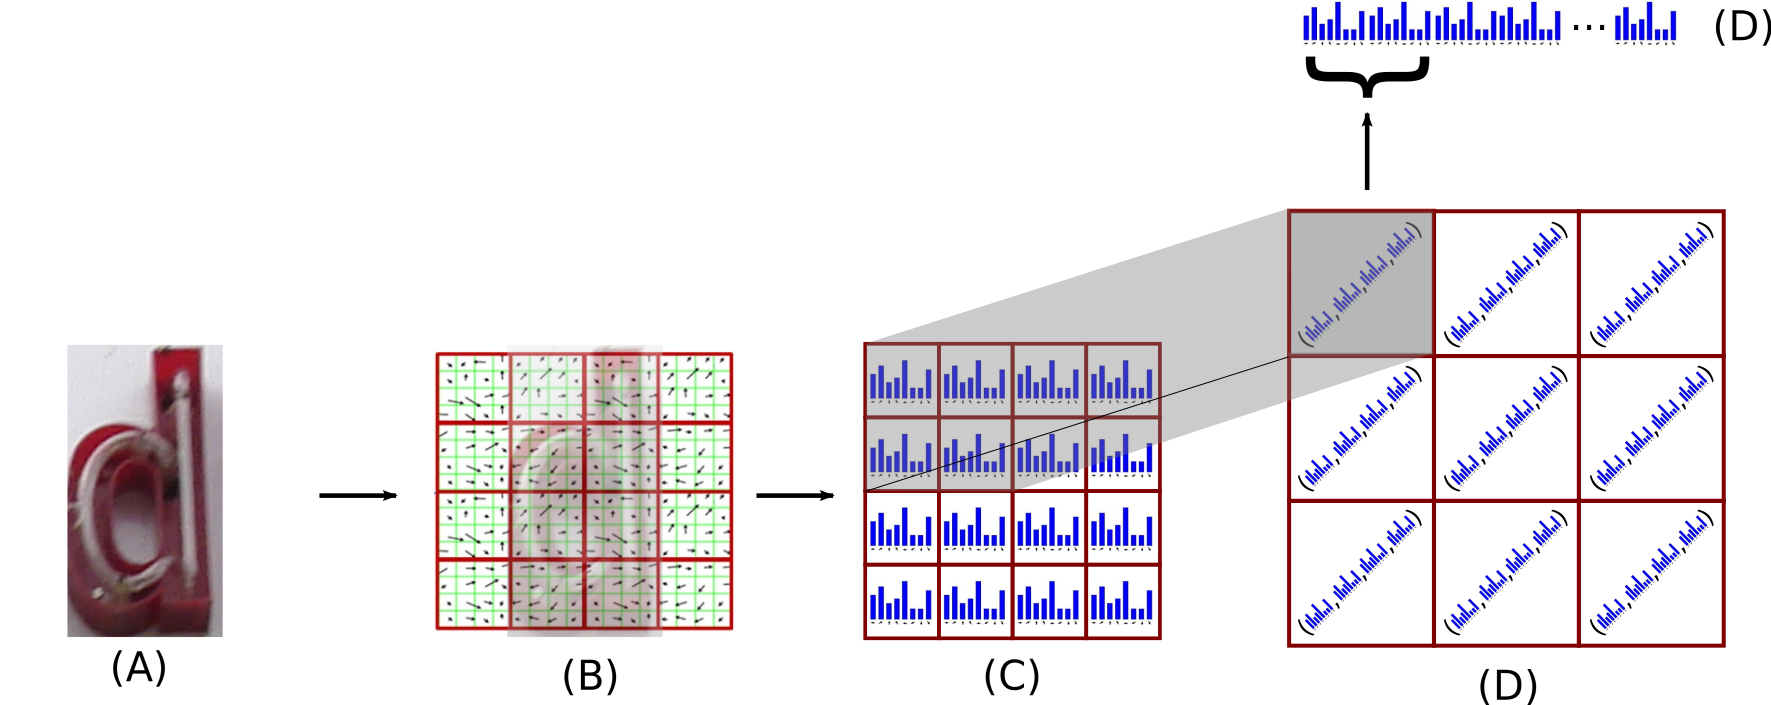
\includegraphics[scale=0.27]{img/hog/hog.png} }
			\caption[Extracción HOG]{Formación del vector de características HOG}
			\label{fig: Vector HOG}
		\end{figure}

	
	%\input{capitulo2/recon_objetos.tex}
